\documentclass{article}
\usepackage[utf8]{inputenc}

\title{\Huge IEL\\Semestrální projekt}
\author{\huge Petr Křehlík\\\Large xkrehl04}
\date{\Large 10.12.2017}

\usepackage{natbib}
\usepackage{graphicx}
\usepackage{comment}
\usepackage{amsmath}

\everymath=\expandafter{\the\everymath\displaystyle}

\usepackage{tikz}


\newcommand*\circled[1]{\tikz[baseline=(char.base)]{
            \node[shape=circle,draw,inner sep=2pt] (char) {#1};}}

\begin{comment}
E	B	E	E	B
\end{comment}

\begin{document}

\maketitle

\pagebreak

\begin{large}

\section{(2 body)}



    Stanovte napětí $U_{R1}$ a proud $I_{R1}$. Použijte metodu postupného zjednodušování obvodu.\\~\\ 
    Zadání E\\
    $U_1=115V$
    $U_2=55V$\\
    $R_1=485\Omega$
    $R_2=660\Omega$
    $R_3=100\Omega$
    $R_4=340\Omega$\\
    $R_5=575\Omega$
    $R_6=815\Omega$
    $R_7=255\Omega$
    $R_8=225\Omega$


\begin{center}
    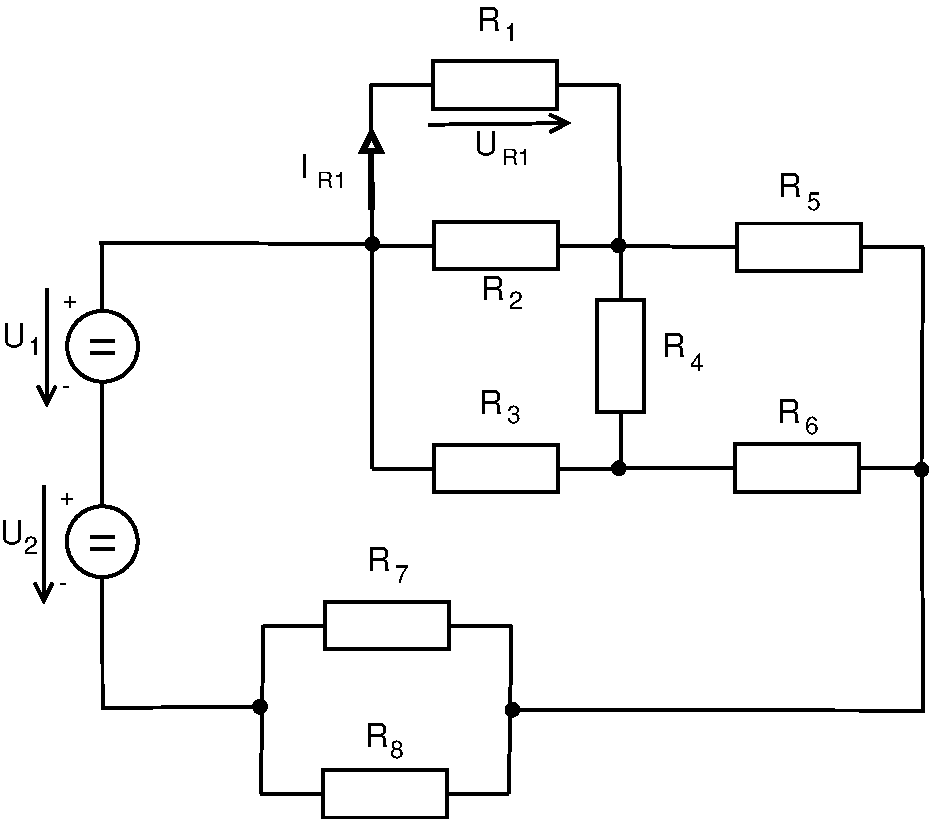
\includegraphics[scale=0.5]{Pr1/Pr1_2017.pdf}
\end{center}


    $R_{12}=\frac{R_1*R_2}{R_1+R_2}=\frac{485*660}{485+660}=279.5633\Omega\;\text{;paralelní zapojení}$\\

    $U=U_1+U_2=115+55=170V\;\text{;sériové zapojení}$\\

    $R_{78}=\frac{R_7*R_8}{R_7+R_8}=\frac{255*225}{255+225}=119.5313\Omega\;\text{;paralelní zapojení}$


\newpage

\begin{center}
    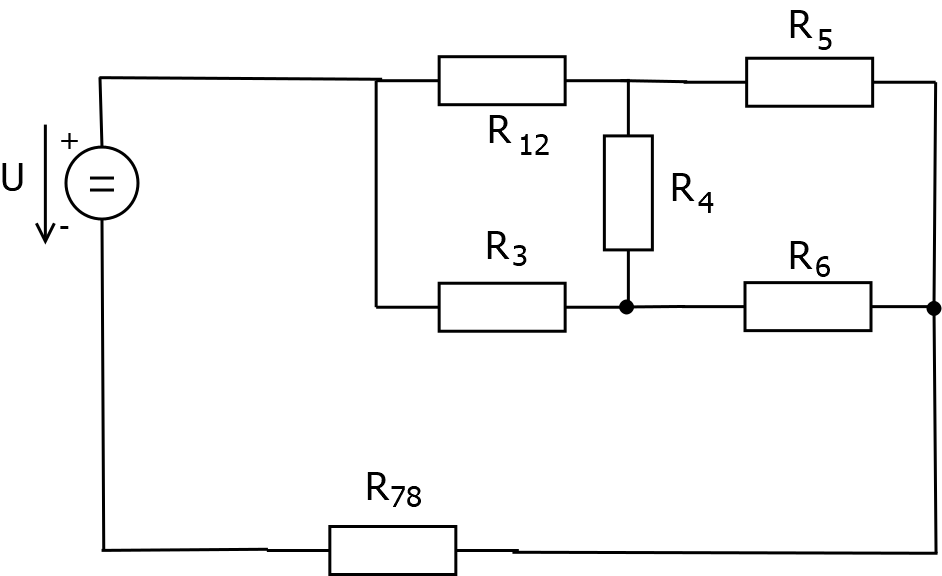
\includegraphics[scale=0.3]{Pr1/Pr1_2.png}
\end{center}


    Trojúhelník-hvězda\\~\\
    $R_A=\frac{R_{12}*R_3}{R_{12}+R_3+R_4}=\frac{279.5633*100}{279.5633+100+340}=38.8518\Omega$\\
    $R_B=\frac{R_{12}*R_4}{R_{12}+R_3+R_4}=\frac{279.5633*340}{279.5633+100+340}=132.0961\Omega$\\
    $R_C=\frac{R_3*R_4}{R_{12}+R_3+R_4}=\frac{100*340}{279.5633+100+340}=47.2509\Omega$


\begin{center}
    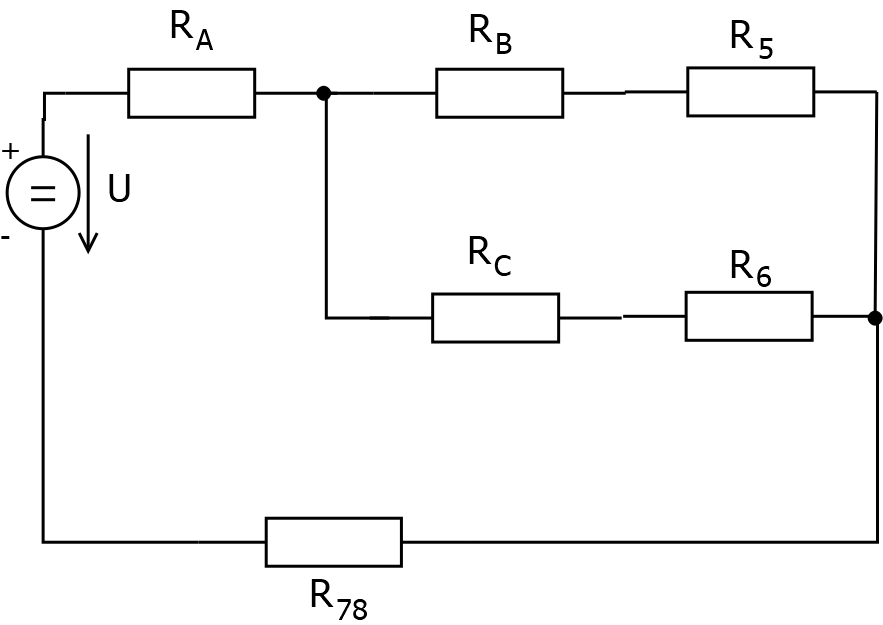
\includegraphics[scale=0.3]{Pr1/Pr1_3.png}
\end{center}


    $R_{B5}=R_B+R_5=132.0961+575=707.0961\Omega\;\text{;sériové zapojení}$
    
    $R_{C6}=R_C+R_6=47.2509+845=892.2509\Omega\;\text{;sériové zapojení}$


\begin{center}
    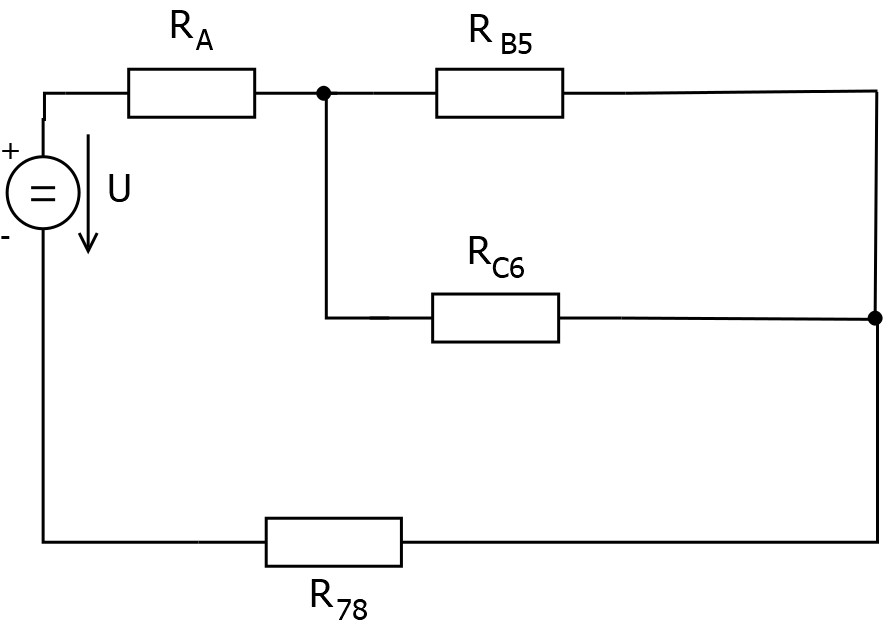
\includegraphics[scale=0.3]{Pr1/Pr1_4.png}
\end{center}


    $R_{B5C6}=\frac{R_{B5}*R_{C6}}{R_{B5}+R_{C6}}=\frac{707.0961*892.2509}{707.0961+892.2509}=392.4780\Omega\;\text{;paralelní zapojení}$


\begin{center}
    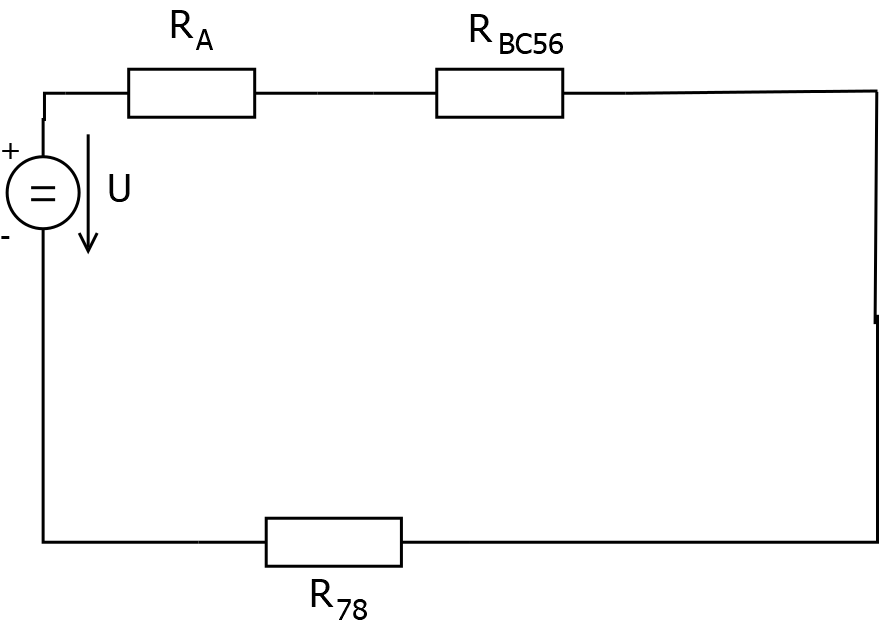
\includegraphics[scale=0.3]{Pr1/Pr1_5.png}
\end{center}


    $R_{EKV}=R_A+R_{B5C6}+R_{78}=38.8518+392.4780+119.5313=550.8611\Omega\;\text{;sériové zapojení}$


\begin{center}
    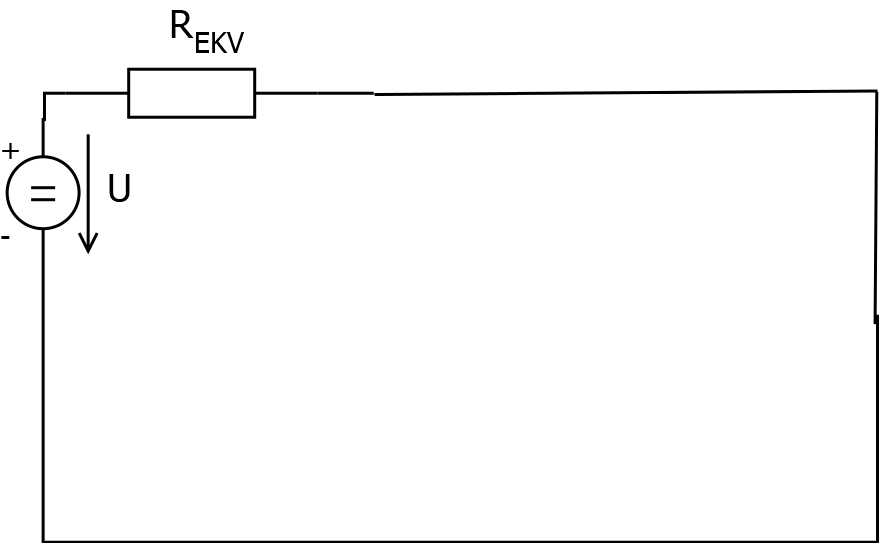
\includegraphics[scale=0.3]{Pr1/Pr1_6.png}
\end{center}


    $I=\frac{U}{R}=\frac{170}{550.8611}=0.3086A$\\
    
    Zpětné skládání obvodu\\
    
    $U_{R_A}=I*R_A=0.3086*38.8518=11.9897V$
    
    $U_{R_{BC56}}=I*R_{BC56}=0.3086*392.4780=121.1187V$
    
    $U_{R_78}=I*R_78=0.3086*119.5313=36.8874V$


\begin{center}
    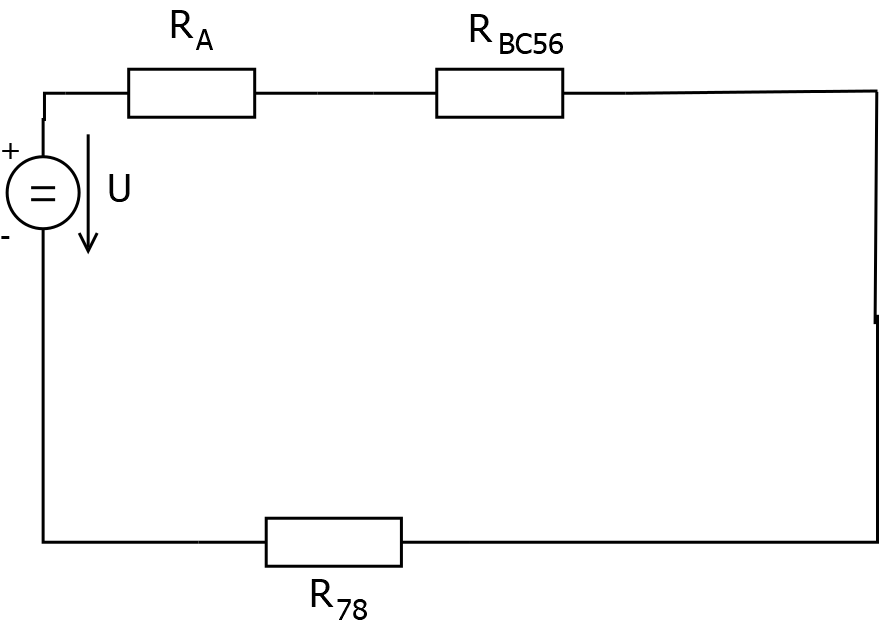
\includegraphics[scale=0.3]{Pr1/Pr1_5.png}
\end{center}

\newpage


    $U_{R_{BC56}}=U_{R_{B5}}=U_{R_{C6}}$\\
    
    $I_{R_{B5}}=\frac{U_{R_{B5}}}{R_{B5}}=\frac{121.1187}{707.0961}=0.1713A$\\
    
    $I_{R_{C6}}=\frac{U_{R_{C6}}}{R_{C6}}=\frac{121.1187}{892.2509}=0.1357A$\\


\begin{center}
    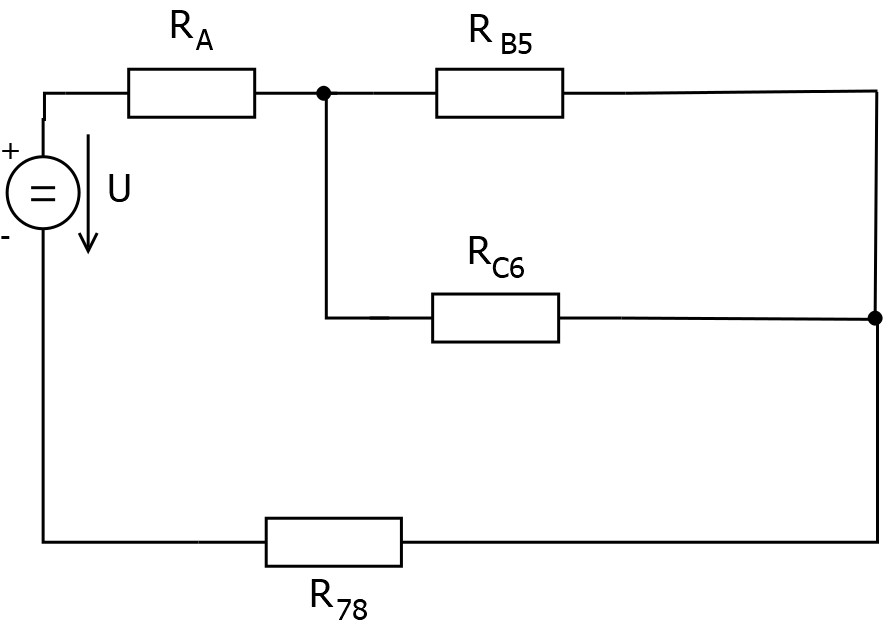
\includegraphics[scale=0.3]{Pr1/Pr1_4.png}
\end{center}


    $I_{R_{B5}}=I_{R_{B}}=I_{R_{5}}$
    
    $I_{R_{C6}}=I_{R_{C}}=I_{R_{6}}$\\
    
    $U_{R_{B}}=I_{R_{B}}*R_{B}=0.1713*132.0961=22.6281V$
    
    $U_{R_{5}}=I_{R_{5}}*R_{5}=0.1713*575=98.4975V$
    
    $U_{R_{C}}=I_{R_{C}}*R_{C}=0.1357*47.2509=6.4120V$
    
    $U_{R_{6}}=I_{R_{6}}*R_{6}=0.1357*815=110.5955V$


\begin{center}
    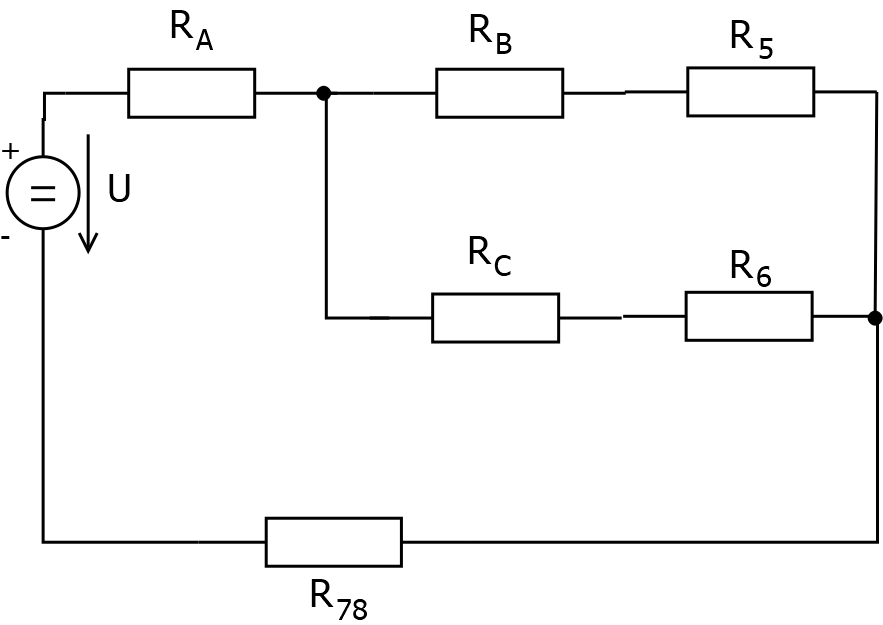
\includegraphics[scale=0.3]{Pr1/Pr1_3.png}
\end{center}


    $U_{R_{12}}+U_{R_5}+U_{R_{78}}-U=0\Rightarrow U_{R_{12}}=U-U_{R_5}-U_{R_{78}}$
    
    $U_{R_{12}}=170-98.4975-36.8874=34.6151V$\\
    
    
    


\begin{center}
    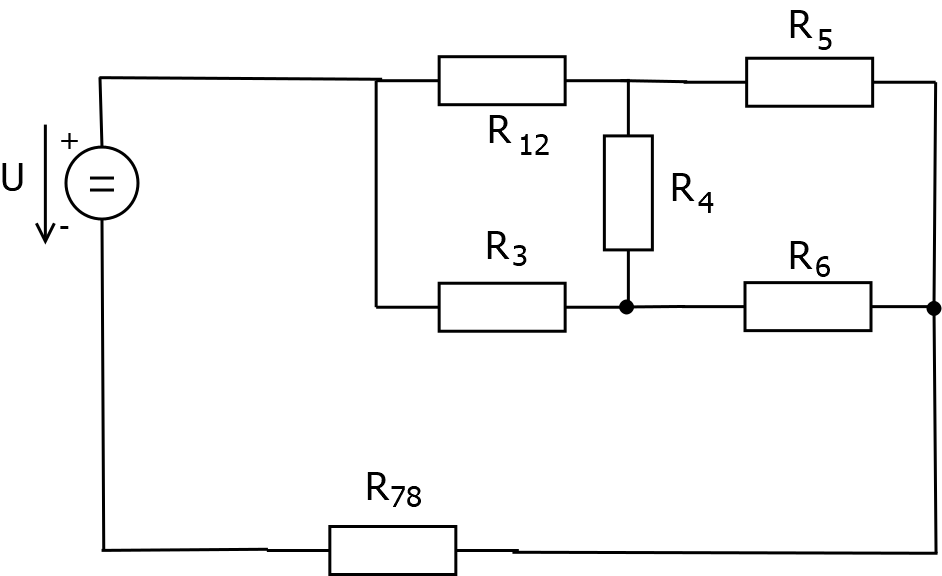
\includegraphics[scale=0.3]{Pr1/Pr1_2.png}
\end{center}

\newpage


    $U_{R_{12}}=U_{R_1}=U_{R_{2}}$\\
    
    \underline{$U_{R_1}=34.6151V$}\\
    
    $I_{R_1}=\frac{U_{R_1}}{R_1}=\frac{34.6151}{485}=0.0713A$\\
    
    \underline{$I_{R_1}=0.0713A$}
    


\begin{center}
    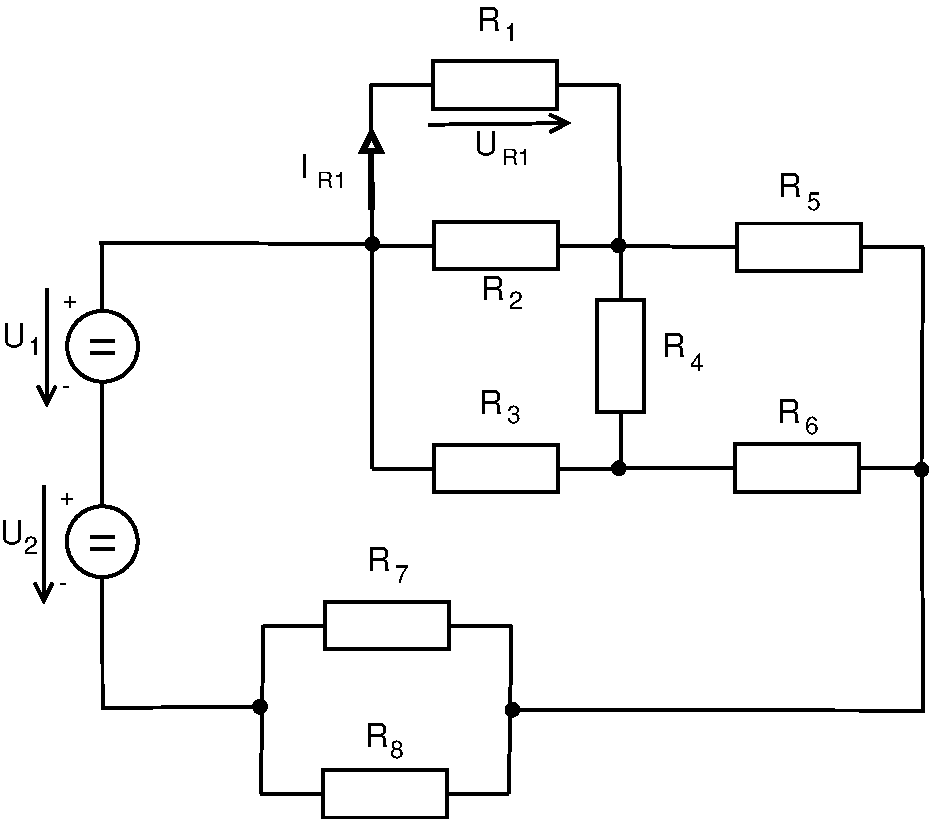
\includegraphics[scale=0.6]{Pr1/Pr1_2017.pdf}
\end{center}

\newpage

\section{(1 bod)}


    Stanovte napětí $U_{R_3}$ a proud $I_{R_3}$. Použijte metodu Théveninovy věty.\\~\\
    Zadání B\\
    $U_1=100V$
    $U_2=50V$\\
    $R_1=310\Omega$
    $R_2=610\Omega$
    $R_3=220\Omega$
    $R_4=570\Omega$
    


\begin{center}
    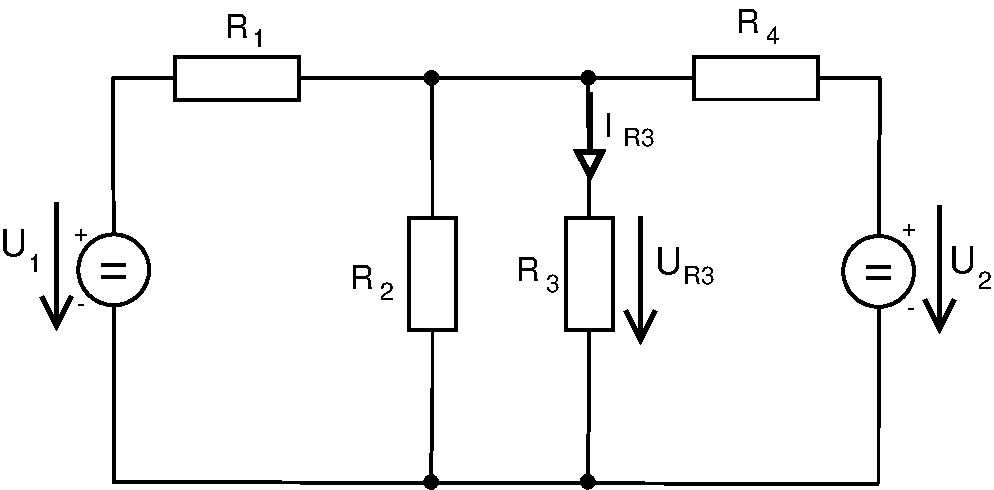
\includegraphics[scale=0.6]{Pr2/Pr2_2017.pdf}
\end{center}


    Nejprve zjednodušíme paralelní odpory $R_2$ a $R_3$.\\
    
    $R_{23}=\frac{R_2*R_3}{R_2+R_3}$\\
    
    Vytvoříme náhradní obvod s $U_i$, $R_i$ a $R_3$.\\


\begin{center}
    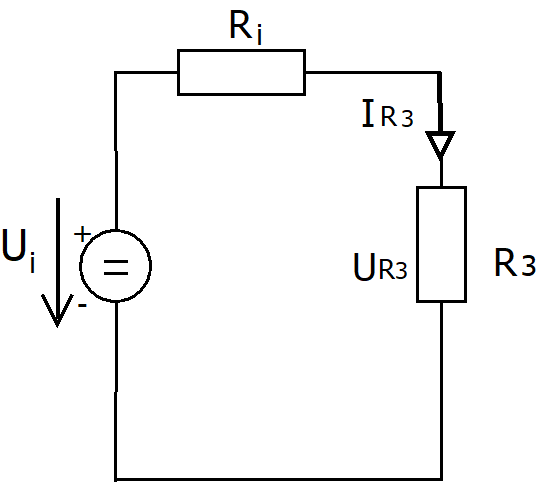
\includegraphics[scale=0.3]{Pr2/Pr2_2017_2.png}
\end{center}

\newpage


    Překreslíme obvod bez $R_3$  a zdroje nahradíme zkratem.
    Spočítáme celkový odpor mezi svorkami.
    $R_i=\frac{R_1*R_4}{R_1+R_4}$


\begin{center}
    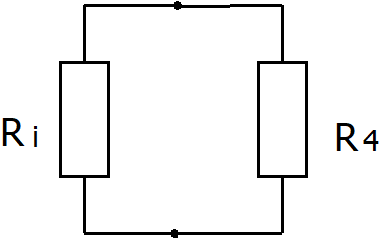
\includegraphics[scale=0.3]{Pr2/Pr2_2017_3.png}
\end{center}


    Překreslíme obvod bez $R_3$ a určíme napětí "naprázdno".\\


\begin{center}
    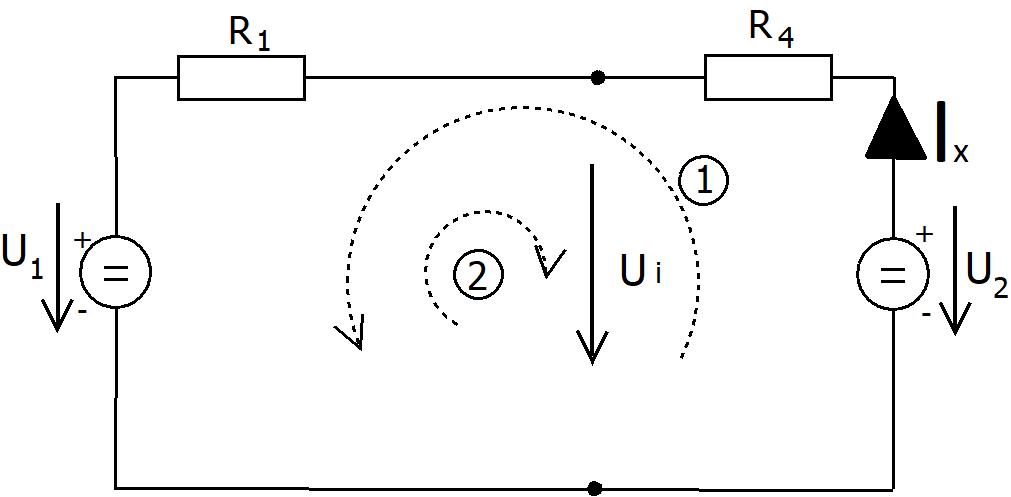
\includegraphics[scale=0.3]{Pr2/Pr_2_3.png}
\end{center}


    \circled{1} $R_1*I_X+R_4*I_X+U_1-U_2=0$
    
    $I_X=\frac{U_2-U_1}{R_1+R_4}$\\
    
    \circled{2} $-R_1*I_X+U_i-U_1=0$\\
    
    $U_i=U_1+R_1*I_X$\\
    
    $I_{R_{23}}=\frac{U_i}{R_i+R_{23}}$\\
    
    $U_{R_{23}}=I_{R_{23}}*R_{23}$\\
    \newpage
    Dosazení:\\
    
    $I_{R_{23}}=\frac{U_1+R_1*\frac{U_2-U_1}{R_1+R_4}}{\frac{R_1*R_4}{R_1+R_4}+\frac{R_2*R_3}{R_2+R_3}}=\frac{100+310*\frac{50-100}{310+570}}{\frac{310*570}{310+570}+\frac{610*220}{610+220}}=0.2272A$\\
    
   
    
    $U_{R_{23}}=I_{R_{23}}*R_{23}=0.2272*\frac{610*220}{610+220}=\underline{36.7488V}$
    
    \underline{$U_{R_{23}}=U_{R_3}$}\\
    
    $I_{R_3}=\frac{U_{R_3}}{R_3}=\frac{36.7488}{220}=\underline{0.1670A}$
    
    


\newpage

\section{(2body)}


    Stanovte napětí $U_{R_5}$ a proud $I_{R_5}$. Použijte metodu uzlových napětí $(U_A, U_B, U_C)$.\\~\\
    Zadání E\\
    $U_1=135V$\\
    $I_1=0.55A$
    $I_2=0.65A$\\
    $R_1=52\Omega$
    $R_2=42\Omega$
    $R_3=52\Omega$
    $R_4=42\Omega$
    $R_5=21\Omega$


\begin{center}
    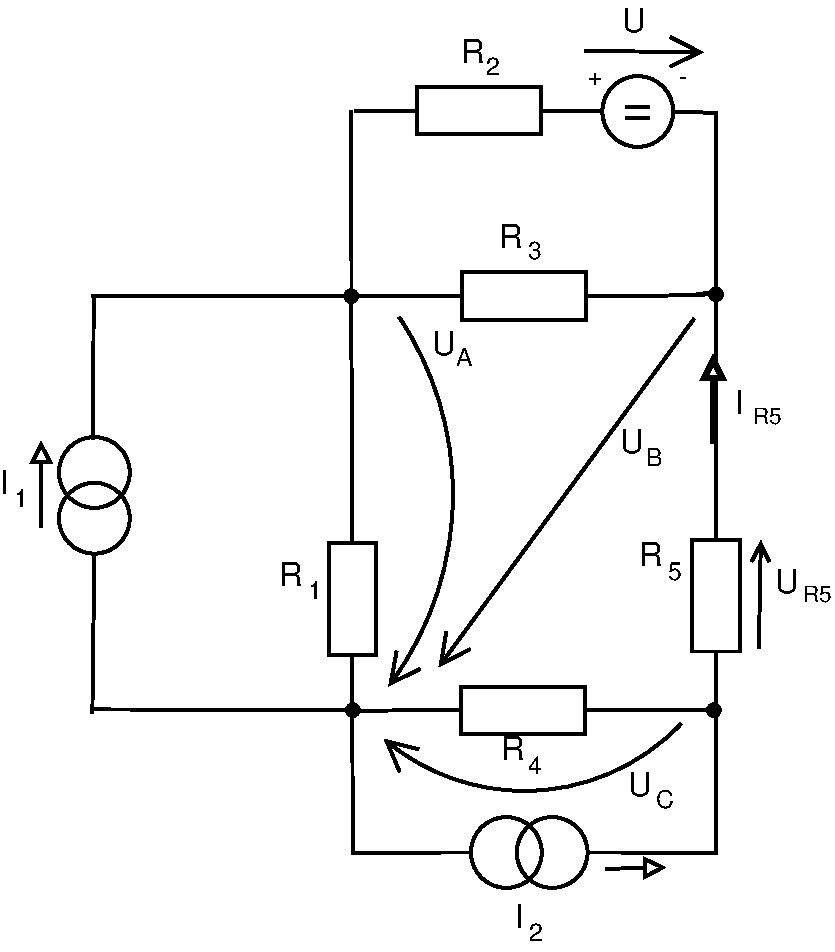
\includegraphics[scale=0.6]{Pr3/Pr3_2017.pdf}
\end{center}
    Překreslíme napěťové zdroje na proudové a odpory, který byly k zdroji v sérii překreslíme na paralelní.
    Odpory nahradíme substitucí $G=\frac{1}{R}$
\begin{center}
    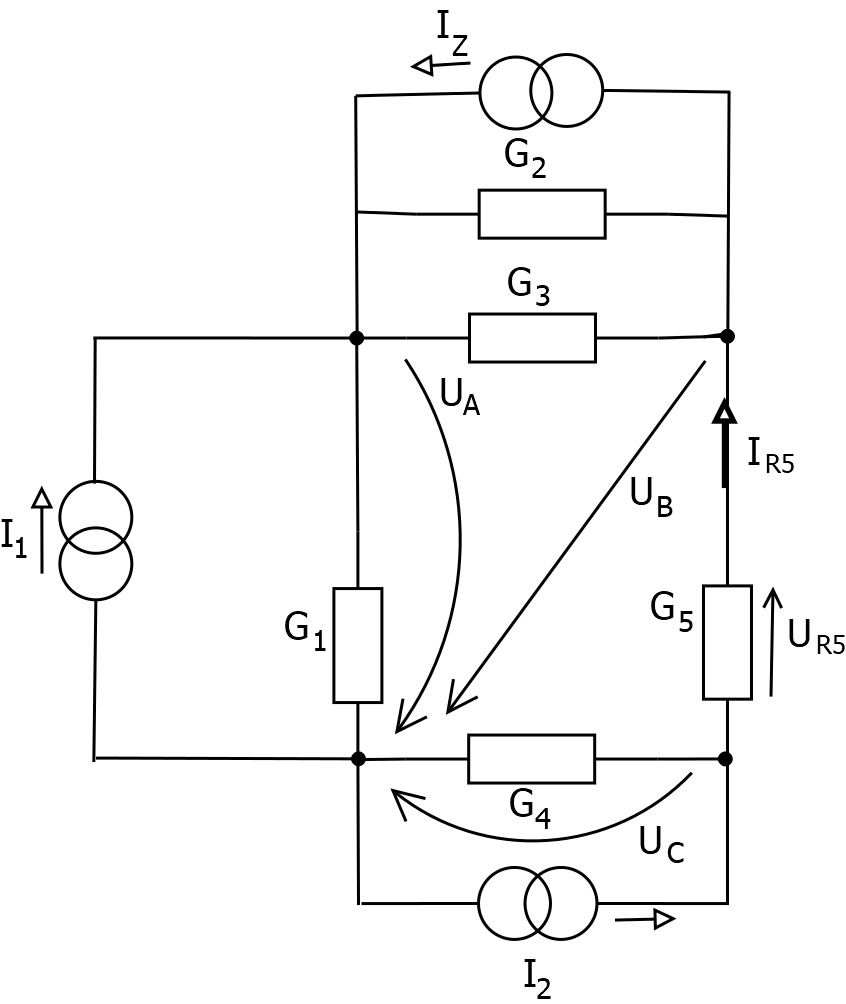
\includegraphics[scale=0.3]{Pr3/Pr3_2.png}
\end{center}
    Dopočítáme $I_Z=\frac{U}{R_2}=\frac{135}{42}=3.2142A$\\
    Sestavíme matici pro uzly $U_A$, $U_B$ a $U_C$ tak, že každý sloupec a řádek představuje uzlové napětí a jaké prvky mají společné.\\
   $ \begin{pmatrix}
    &U_A & U_B & U_C\\
    U_A&G_1+G_2+G_3 & -G_2-G_3 & 0\\
    U_B&-G_2-G_3 & G_2+G_3+G_5 & -G_5\\
    U_C&0 & -G_5 & G_4+G_5
    \end{pmatrix} $ \\Doplníme hodnoty a vypočítáme determinant\\
    Det
    $\begin{pmatrix}
    \frac{17}{273} & -\frac{47}{1092} & 0\\~\\
    -\frac{47}{1092}& \frac{33}{364} & -\frac{1}{21}\\~\\
    0 & -\frac{1}{21} & \frac{1}{14}
    \end{pmatrix}=1.2972*10^{-4}$
    \\Vypočítáme determinant matice a poté Sarussovým pravidlem vypočítáme determinanty pro jednotlivá napětí. \\Vždy dosadíme 
    $\begin{pmatrix}
    I_1+I_{Z}\\
    -I_Z\\
    I_2
    \end{pmatrix}$za sloupec a vypočítáme determinant.\\
    $U_B:$\\~\\
    $\begin{pmatrix}
    \frac{17}{273} & 3.7642 & 0\\~\\
    -\frac{47}{1092}& -\frac{45}{14} & -\frac{1}{21}\\~\\
    0 & 0.65 & \frac{1}{14}
    \end{pmatrix}=-0.000797$\\
    $U_B=\frac{det(B)}{det}=\frac{-0.000797}{1.2972*10^{-4}}=-6.1438V$\\~\\
    $U_C:$\\~\\
    $\begin{pmatrix}
    \frac{17}{273} & -\frac{47}{1092} & 3.7642\\~\\
    -\frac{47}{1092}& \frac{33}{364} & -\frac{45}{14}\\~\\
    0 & -\frac{1}{21} & 0.65
    \end{pmatrix}=0.000649$\\~\\
    $U_C=\frac{det(C)}{det}=\frac{0.000649}{1.2972*10^{-4}}=5.0031V$\\~\\
    $U_{R_5}=U_B-U_C=\underline{-11.1469V}$\\
    $I_{R_5}=\frac{U_{R_5}}{R_5}=\underline{-0.5308A}$\\
  
    
\pagebreak

\section{(2body)}
\begin{flushleft}

Pro napájecí napětí platí: $u1 = U1*sin(2\pi f t), u2 = U2*sin(2\pi f t)$.
Ve vztahu pro napětí $uC1 = UC1*sin(2\pi f t+\omega C1)$ určete $|UC1|$ a $\omega C1$. Použijte metodu smyčkových proudů.
Pozn: Pomocné "směry šipek napájecích zdrojů platí pro speciální časový okamžik $(t =\pi/2\omega)$."\medskip

Zadání E\medskip

$U_1=50V$
$U_2=30V$\\
$R_1=14\Omega$
$R_2=13\Omega$
$R_3=14\Omega$\\
$L_1=130mH$
$L_2=60mH$\\
$C_1=100uF$
$C_2=65uF$\\
$f=90Hz$

\begin{center}
    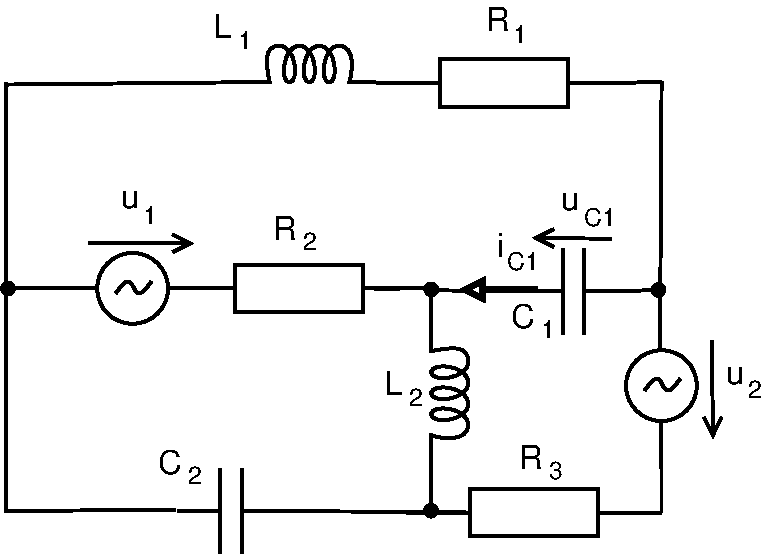
\includegraphics[scale=0.6]{Pr4/Pr4_2017.pdf}
\end{center}

Překreslíme obvod s nahrazením všech součástek za odpory a naznačíme smyčky.

\begin{center}
    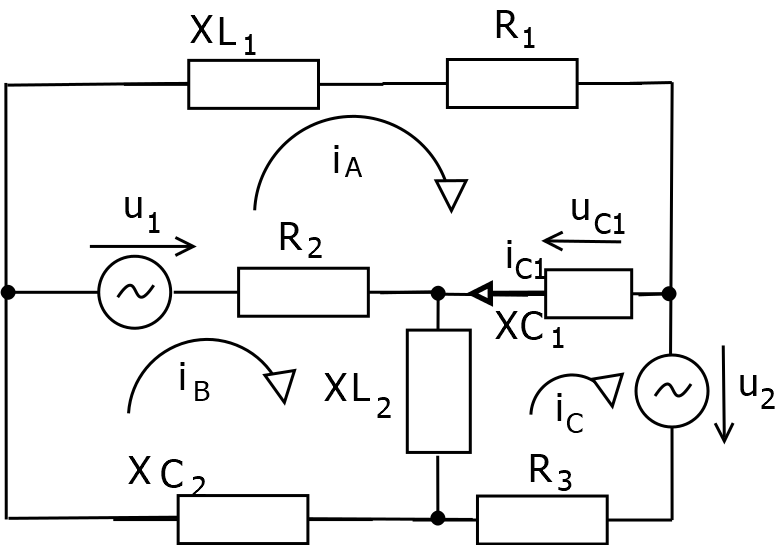
\includegraphics[scale=0.3]{Pr4/Pr4_2.png}
\end{center}
Nejdříve určíme $\omega=2\pi f=2\pi90=180\pi\;rad/s$\\~\\

Velikost imaginárních odporů určíme výpočtem reaktancí:\\~\\
$X_{L_1}=j*\omega*L_1=j*\omega*0.13=73.5132j\Omega$

$X_{L_2}=j*\omega*L_2=j*\omega*0.06=33.9292j\Omega$

$X_{C_1}=-\frac{j}{\omega*C_1}=-\frac{j}{180\pi*100*10^{-6}}=-17.6839j\Omega$

$X_{C_2}=-\frac{j}{\omega*C_2}=-\frac{j}{180\pi*65*10^{-6}}=-27.20597j\Omega$\\~\\

Sestavíme rovnice smyček pomocí 2. Kirchhoffova zákona:\\

$(X_{L_1}+R_1)*I_A+X_{C_1}*(I_A-I_C)+R_2*(I_A-I_B)=U_1$
$R_2*(I_B-I_A)+X_{L_2}*(I_B-I_C)+X_{C_2}*I_B=-U_1$
$R_3*I_C+X_{L_2}*(I_C-I_B)+X_{C_1}*(I_C-I_A)=-U_2$

Dosadíme do matice (sloupce představují $I_A, I_B, I_C$):\\
$\begin{pmatrix}
X_{L_1}+R_1+X_{C_1}+R_2 & -R_2 & -X_{C_1}\\
-R_2 & R_2+X_{L_2}+X_{C_2} & -X_{L_2}\\
-X_{C_1} & -X_{L_2} & X_{C_1}+X_{L_2}+R_3
\end{pmatrix}$\\

Dosadíme číselné hodnoty:\\
$\begin{pmatrix}
27+55.8293j & -13 & 17.6839j\\
-13 & 13+6.72323j & -33.9292j\\
17.6839j & -33.9292j & 14+16.2453j
\end{pmatrix}$\\

Vypočítáme determinant matice:

$det=2101.05803+75933.8891j$
\newpage
Vypočítáme determinant pro $I_C$ dosazením do třetího sloupce
$\begin{pmatrix}
U_1\\-U_1\\-U_2
\end{pmatrix}$Dosadíme:
$\begin{pmatrix}
50\\-50\\-30
\end{pmatrix}$\\~\\

$det(I_C)=\begin{pmatrix}
27+55.8293j & -13 & 50\\
-13 & 13+6.72323j & -50\\
17.6839j & -33.9292j & -30
\end{pmatrix}=\newline
=106457.41737-50969.6833j$\\~\\

$I_C=\frac{det(I_C)}{det}=\frac{106457.41737-50969.6833j}{2101.05803+75933.8891j}=\newline=-0.63196174-1.4194612jA$\\~\\

$det(I_A)=\begin{pmatrix}
27+55.8293j & 50 & 17.6839j\\
-13 & -50 & -33.9292j\\
17.6839j & -30 & 14+16.2453j
\end{pmatrix}\newline
=106739.50396-71038.151j$\\~\\

$I_A=\frac{det(I_A)}{det}=\frac{106739.50396-71038.151j}{2101.05803+75933.8891j}=\newline=-0.89594553-1.4304804jA$\\~\\

$U_{C_1}=X_{C_1}*(I_C-I_A)=-17.6839j*((-0.63196174-1.4194612j)-(-0.89594553-1.4304804j))=0.194862-4.66826j$\\~\\

$|U_{C_1}|=\sqrt{0.194862^2+4.66826^2}=\underline{4.67233V}$\\~\\

$\phi=-arctg(\frac{Img U_{C_1}}{Re U_{C_1}})*\frac{\pi}{180}=-arctg(\frac{4.66826}{0.194862}*\frac{\pi}{180})=\underline{-0.396032 rad}$

\newpage

\section{(2 body)}

...

\newpage


Výsledky:


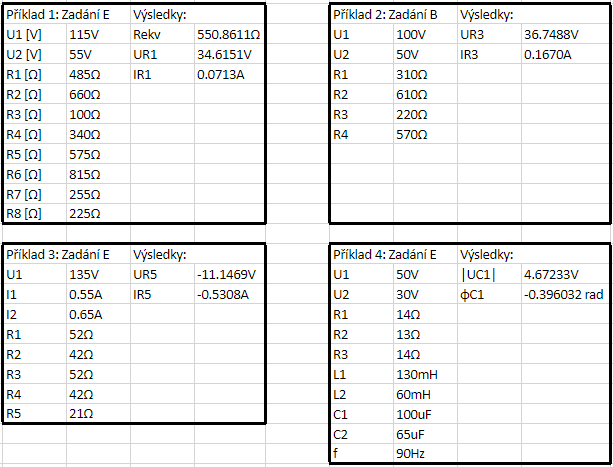
\includegraphics[scale=1]{vys.PNG}


\end{flushleft}

\end{large}

\end{document}
